\documentclass[letterpaper, 10 pt, conference]{ieeeconf}  % Comment this line out
                                                          % if you need a4paper
%\documentclass[a4paper, 10pt, conference]{ieeeconf}      % Use this line for a4
                                                          % paper

\IEEEoverridecommandlockouts                              % This command is only
                                                          % needed if you want to
                                                          % use the \thanks command
\overrideIEEEmargins
% See the \addtolength command later in the file to balance the column lengths
% on the last page of the document



% The following packages can be found on http:\\www.ctan.org
%\usepackage{graphics} % for pdf, bitmapped graphics files
\usepackage[pdftex]{graphicx}
\usepackage{url}
%\usepackage{epsfig} % for postscript graphics files
%\usepackage{mathptmx} % assumes new font selection scheme installed
%\usepackage{times} % assumes new font selection scheme installed
%\usepackage{amsmath} % assumes amsmath package installed
%\usepackage{amssymb}  % assumes amsmath package installed
%\usepackage{multicol}

\title{\LARGE \bf High-Accuracy 3D Sensing for Mobile Manipulation:\\Improving Object Detection and Door Opening}

\author{ \parbox{6.5in}{\centering Morgan Quigley, Siddharth Batra, Stephen Gould, Ellen Klingbeil,\\Quoc Le, Ashley Wellman, and Andrew Y. Ng\\
         Computer Science Department\\
         Stanford University\\
         {\tt\scriptsize\{mquigley, sidbatra, sgould, ellenrk, quocle, wellman, ang\}@cs.stanford.edu}}
}

\begin{document}

\maketitle
\thispagestyle{empty}
\pagestyle{empty}


%%%%%%%%%%%%%%%%%%%%%%%%%%%%%%%%%%%%%%%%%%%%%%%%%%%%%%%%%%%%%%%%%%%%%%%%%%%%%%%%
\begin{abstract}

High-resolution 3D scanning can improve the performance of object detection and
door opening, two tasks critical to the operation of mobile manipulators in
cluttered homes and workplaces. We discuss how high-resolution depth
information can be combined with visual imagery to improve the performance
of object detection beyond what is (currently) achievable with 2D images alone,
and we present door-opening and inventory-taking experiments.

\end{abstract}


%%%%%%%%%%%%%%%%%%%%%%%%%%%%%%%%%%%%%%%%%%%%%%%%%%%%%%%%%%%%%%%%%%%%%%%%%%%%%%%%
\section{INTRODUCTION}

%Thanks to achievements in mechanical and electrical engineering, large mobile
%manipulators have the physical capability of performing useful tasks in
%uncontrolled, cluttered environments. Tele-operated mobile manipulators are
%currently employed to perform manipulation tasks in bomb disposal and tactical
%reconnaissance situations, and intricate manipulation tasks have been performed
%for decades by robots on production lines. However, mobile manipulators have
%  not seen widespread use outside of these highly specialized domains.

%If mobile manipulators could be automated in uncontrolled environments, they
%could prove useful in areas such as home and office automation, sanitation,
%elder care, and security, among others.  Indeed, the exciting potential of
%large mobile manipulators, humanoid or not, has been one of the great dreams of
%AI for decades, and large mobile manipulators for homes and offices are
%currently being investigated by a number of research groups. Unfortunately, 

%Typical homes and offices are difficult places for large mobile manipulators to
%operate, as they are filled with clutter and constantly changing.
In this
paper, we propose employing high-resolution 3D sensing on mobile manipulators.
%For our experiments, we constructed a medium-range laser line triangulation
%system.
Just as the change from sonar-based sensing to laser-based sensing enabled
drastic improvement of SLAM in mobile robotics, we propose that dramatically
improving the quality of depth estimation on mobile manipulators can enable new
classes of algorithms and higher levels of performance (Figure
\ref{fig:coffee_mug}).  In support of this idea, we present two scenarios
where high-accuracy 3D data proves useful to large mobile manipulators
operating in cluttered environments.

The first scenario involves object detection. In many tasks, a mobile
manipulator needs to search for an object class in a cluttered environment.
This problem is challenging when only visual information is given to the
system: variations in background, lighting, scene structure, and object
orientation exacerbate an already-difficult problem. We demonstrate that
augmenting state-of-the-art computer vision techniques with high-resolution 3D
information results in higher precision and recall than is currently achievable
by either modality alone.

The second scenario involves manipulator trajectory planning. We demonstrate
closed-loop perception and manipulation of door handles using information from
both visual images and the 3D scanner. The high-resolution 3D information helps
ensure that the trajectory planner keeps the manipulator clear of the door
while still contacting the door handle.

\begin{figure}[t]
\begin{center}
  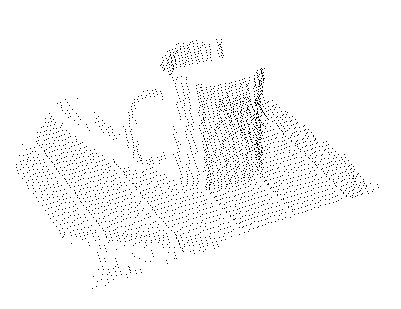
\includegraphics[width=2.0in]{mug_closeup_1.jpg} \\
  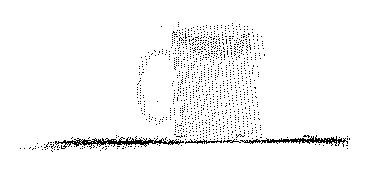
\includegraphics[width=2.0in]{mug_closeup_2.jpg} \\
  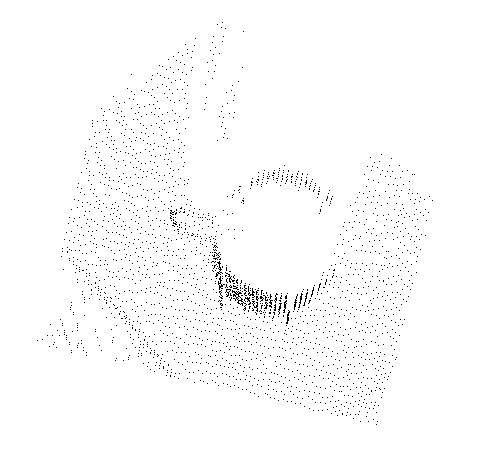
\includegraphics[width=2.0in]{mug_closeup_3.jpg}
\end{center}
\caption{Several off-axis views of a raw scan of a coffee mug obtained by our scanner from 1.2 meters away. The 5mm-thick handle is prominently visible. Approximately 1000 points of the scan are on the surface of the coffee mug, despite the fact that it comprises only 5\% of the horizontal field-of-view of scan.}
\label{fig:coffee_mug}
\end{figure}

We then present an application experiment which combines these capabilities to
perform a simple inventory-control task. The mobile manipulator enters several
offices and searches for an object class, recording the detected locations.

%Large mobile manipulators operating in uncontrolled environments must be able
%to perceive the world around them in order to safely and usefully interact with
%it. For example, a manipulator must be able to plan a collision-free trajectory
%in order to grasp an item without disturbing nearby objects.  Furthermore,
%mobile manipulators need to recognize target objects in the first place, and
%object recognition in cluttered environments is challenging. Huge variations in
%background, lighting, scene structure, object orientation, etc., exacerbate an
%already-difficult problem. Progress has been made in the computer vision
%community to address some of these issues in some situations; however, a
%robust, general-purpose object recognition system remains an elusive goal.

%In this paper, we propose medium-range laser line triangulation as a means to
%augment state-of-the-art computer vision techniques with depth information. We
%demonstrate that features extracted from highly accurate depthmaps are
%complementary to features extracted from visual images, resulting in higher
%precision and recall than currently achievable by either modality alone. We
%also demonstrate that these highly accurate point clouds are useful in planning
%arm trajectories for mobile manipulators. We show a demonstration
%inventory-control application where these techniques are used in a typical
%cluttered office environment to both improve the reliability of autonomous door
%opening and to catalog instances an object class.

\section{MOTIVATION AND RELATED WORK}

\begin{figure}[t]
\begin{center}
  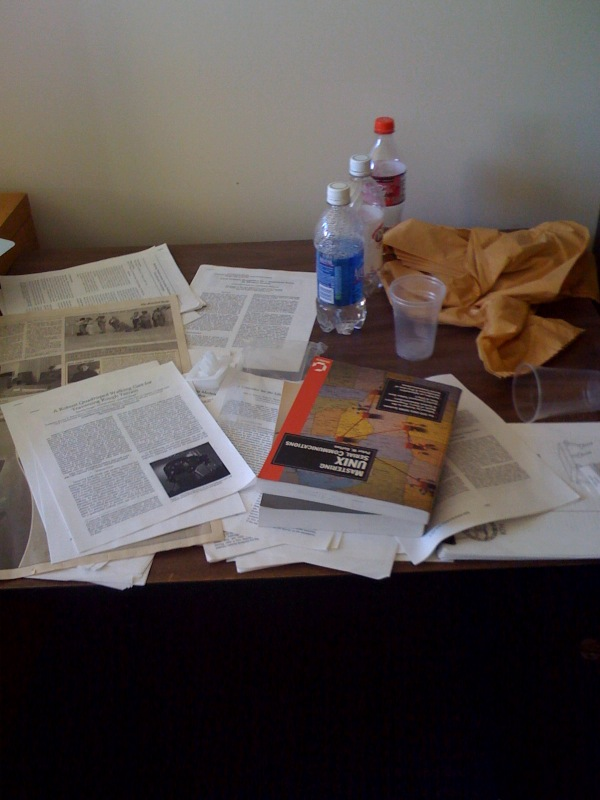
\includegraphics[width=1.6in]{clutter1.jpg} \quad
  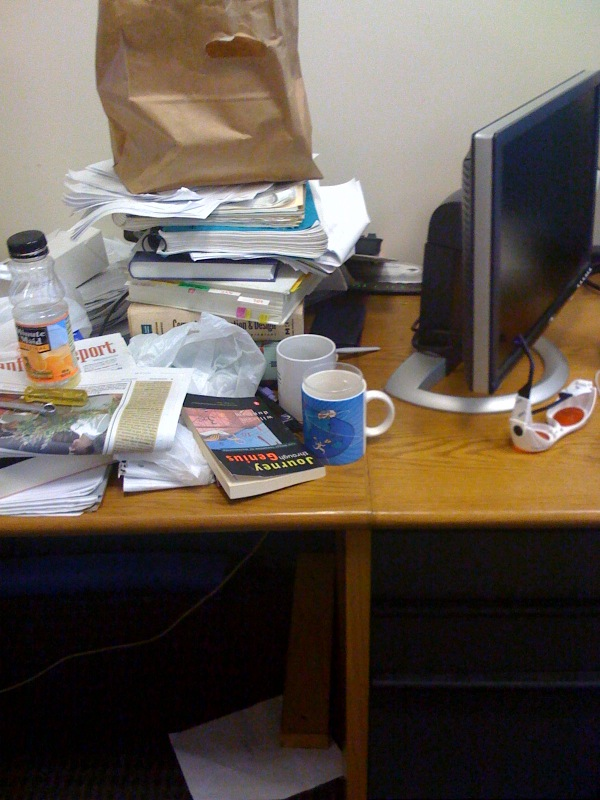
\includegraphics[width=1.6in]{clutter2.jpg}
\end{center}
\caption{Clutter makes scene understanding from only 2D visual images difficult, even in a relatively simple office environment, as many of the strong edges are not those which suggest the 3D structure of the scene.}
\label{fig:clutter}
\end{figure}

%Mobile manipulation involves many subfields of AI, including computer vision,
%robotics, and planning. As a result, mobile manipulators often have more
%comprehensive sensor packages than each of the subfields typically uses in
%isolation (Figure \ref{fig:stair1}). For example, much of the computer vision
%literature has focused on recognizing object classes in 2D visual images. This
%restriction is necessary in many common scenarios, such as datasets acquired
%from the Internet or unaided cameras. However, when computer vision is used in
%mobile manipulation, other sensors are often available on the platform and can
%boost performance over that achievable with current state-of-the-art 2D vision
%algorithms.


%The 2D vision problem is challenging for many reasons, one of which being the
%loss of dimensionality inherent in the image-formation process. Algorithms
%seeking to recognize objects in the world must cope with 2D projection
%either explicitly, by storing and fitting 3D models, or implicitly, by training
%2D classifiers on many views of an object. Inferring an object class from a 2D
%image has had some notable successes, such as face detection. However, the
%ambiguity inherent in many visual images of common cluttered scenes is
%difficult to resolve (Figure \ref{fig:clutter}), and can only be inferred
%through cues such as shading, structure from motion, or prior knowledge, all of
%which are challenging open problems in the general case. Algorithms for
%holistic scene understanding show promise at addressing some of these
%ambiguities for domains like autonomous driving, but the problem still remains
%unsolved in the general case.

Augmenting vision algorithms with 3D sensing has the potential to reduce some
of the difficulties inherent in image-only object recognition. Prior work has
shown that low-resolution depth information can improve object detection by
removing object classifications which are inconsistent with training data
(e.g., objects are usually not floating in the air, and some object classes are
unlikely to be on the floor)~\cite{bib:eccv}.

However, if a depth sensor's noise is comparable to the size of the target
object classes, it will be hard-pressed to provide more than contextual
cues. The difference between a stapler and a coffee mug, for example, is
only several centimeters in each dimension. Indeed, many objects designed for
manipulation by human hands tend to be similarly sized and placed; thus, using
depth information to distinguish among them requires sub-centimeter
accuracy.

%\begin{figure}[t]
%\begin{center}
%  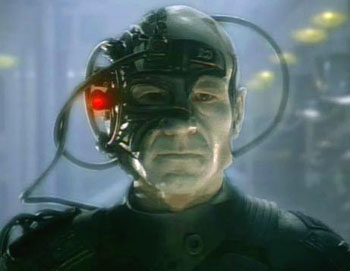
\includegraphics[width=3in]{borg.jpg}
%\end{center}
%\caption{A coffee mug, disposable cup, and stapler next to each other on a table, imaged by each of the modalities discussed above.}
%\label{fig:ranger_comparison}
%\end{figure}

Unfortunately, many current sensing technologies have noise figures on the
centimeter level when measuring from 1-2 meters away. Ranging devices based
on time-of-flight, for example, tend to have centimeter-level noise due to the
extremely short timescales involved \cite{bib:3d-cam-iros06}. Additionally,
time-of-flight ranging systems can introduce depth artifacts correlated with
the reflectance or surface normal of the target object
\cite{bib:noise-of-3d-cams}.

In contrast, the accuracy of passive stereo cameras is limited by the ability
to find precise feature matches. Stereo vision can be significantly improved
using global-optimization techniques\cite{bib:global-stereo}, but the
fundamental problem remains: many surfaces, particularly in artifical
environments, do not possess sufficient texture to permit robust feature
matching (e.g., a blank piece of paper).  Efforts have recently been made to
combine passive stereo with time-of-flight cameras \cite{bib:cam-fusion},
but the resulting noise figures still tend to be larger than what is achievable
using a laser line scanner.

Active vision techniques use yet another approach: they project large patterns
onto the scene using a video projector, and observe deformations of the
patterns in a camera to infer depth \cite{bib:active-vision}.  Besides the
difficulties inherent in overcoming ambient light simultaneously over a large
area, the projected image must be at least roughly focused, and thus depth of
field is limited by the optical geometry. However, this is a field of active
research and great strides have been made in recent years.

This brief summary of the limitations of alternative 3D sensing modalities is
bound to change with the continual progress being made in each of the
respective areas of inquiry. In this paper, we seek to explore the potential
benefits of highly accurate 3D data for mobile manipulators. As other 3D
modalities continue to improve, their data could be used by the algorithms
described in this paper. For the purposes of this study, we have built several
3D laser line triangulation systems to explore how high-quality 3D data can
improve the performance of mobile manipulation.

We selected laser line triangulation because millimeter-level accuracy
is readily achievable. This is on the order of accuracy we have been able to
achieve in sensor-to-manipulator calibration; further increases in
sensing accuracy would thus not necessarily improve manipulation
performance.


Laser line scanners have proven useful in manufacturing, as is well documented
both in the research literature \cite{bib:li-manufacturing-robot} and in the
marketplace \cite{bib:industrial-scanners}. They have been often used
in fixed installations, where objects are placed on a rotary table in
front of the scanner \cite{bib:cvpr-88} or flow by on conveyor belts.  Low-cost
implementations have been designed which rely on a known background pattern
instead of precision hardware \cite{bib:david-scanner}. Triangulation-based
laser scanners have also been used on planetary rovers to model rough terrain
\cite{bib:mars-rover}, to find curbs for autonomous vehicles
\cite{bib:curbfinder} and to model archaelogical sites and works of art
\cite{bib:levoy}.
  
Out-of-the-box triangulation systems are commercially available for
imaging small objects \cite{bib:nextengine}. However, many of these systems
emphasize high accuracy ($<$~0.1mm), often sacrificing
depth of field. To be of most use to a mobile manipulator, the sensor needs to
cover the entire workspace of the manipulator, and ``extra'' sensing range is
helpful in determining how to move the platform so that a nearby object will
enter the workspace of the manipulator.

Although triangulation-based laser scanners have been proposed for mobile
manipulators in the past \cite{bib:door-iros-94}, at time of writing, we are
not aware of implemented systems similar to what we describe in this paper. 

\section{LASER LINE SCANNING FOR ROBOTICS}

Our scanner is intended to complement computer vision systems on mobile
manipulators. As such, we aim to produce a depth estimate for each pixel in the
scene. The resulting images can be considered as having an ``extra" channel
representing each pixel's depth, in addition to the usual RGB- or
monochrome-intensity channels.

\subsection{Fundamentals}

The geometry of the laser-line triangulation scheme is well-studied and only
repeated here for completeness. Many variants of the underlying concepts are
possible. In our scanners, a rotating vertical laser line is directed into the
scene.  An image formed on a rigid, horizontally-offset camera shows a line
which is deformed by the depth variations of the scene (Figures
\ref{fig:sample_line} and \ref{fig:borg2}).  On each scanline of the image, the
centroid of the laser is detected and used to define a ray from the camera
origin through the image plane and into the scene. This ray is intersected with
the plane of laser light defined by the angle of the laser stage, its axis of
rotation, and 3D translation from the laser stage to the camera origin.  The
intersection of the plane and pixel ray produces a single 3D point directly in
the image frame, thus avoiding the depthmap-to-image registration problem.

The vertical angular resolution of the point cloud is limited by the vertical
resolution of the camera. The horizontal resolution is determined by
the the laser's rotation speed, the camera's frame rate, and the field of view.
Depth resolution is determined by a variety of factors: the ratio between the
horizontal resolution of the camera and the field of view, the precision of the
shaft encoder on the laser stage, the ability to achieve horizontal sub-pixel
interpolation, the horizontal offset between the camera and the laser, and the
distance of the object from the camera.

\subsection{Hardware Considerations}

We acquire roughly 600 images during each scan. The camera's field of view is
approximately 70 degrees, and we overscan by 10 degrees to accomodate for the
depth variations of the scene. As a result, the laser line moves approximately
0.15 degrees per frame. 

%We experimented with a number of laser line generators before settling on a
%532nm (green) module. As with any laser device, eye safety is a concern.
%Although the laser diode in our system outputs more power than is permissible
%to be considered eye-safe, the line-generating lens causes the energy to become
%spatially distributed as the distance from the lens increases. The physical
%construction of the robot makes it very difficult for an eye to be closer than
%10cm to the laser (at which point the laser's 90 degree fan angle has caused
%the line to be 20cm long). At that distance, only a small fraction of the
%laser's optical output would be entering the eye. To ensure the safety of
%the device in a real-world implementation, baffles could be added to physically
%ensure such a ``stand-off'' distance.

Our scanner currently requires 6 seconds to gather the images, which are
buffered in RAM on a computer onboard the robot.  Subsequent image processing
and triangulation steps require an additional 4 seconds. Such a slow rate of 
acquisition means that the scanner cannot be used in fast-moving scenes. This
is a fundamental limitation of line scanning; however, additional
implementation effort could result in dramatic speedups, e.g., moving to
(very) high-speed cameras and/or performing the image processing on a graphics
processor (GPU).

\subsection{Calibration}

\begin{figure}[t]
\begin{center}
  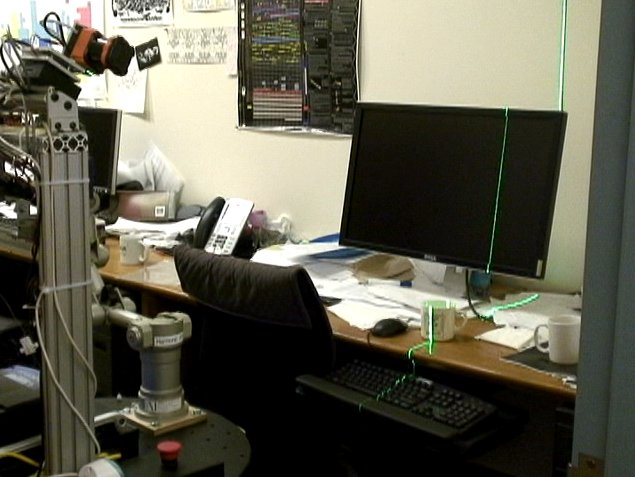
\includegraphics[width=0.83\linewidth]{borg-line.jpg}
\end{center}
\caption{A vertical (green) laser line projected by the robot at left is deformed
as it strikes objects in the scene.}
\label{fig:sample_line}
\end{figure}
\begin{figure}[t]
\begin{center}
  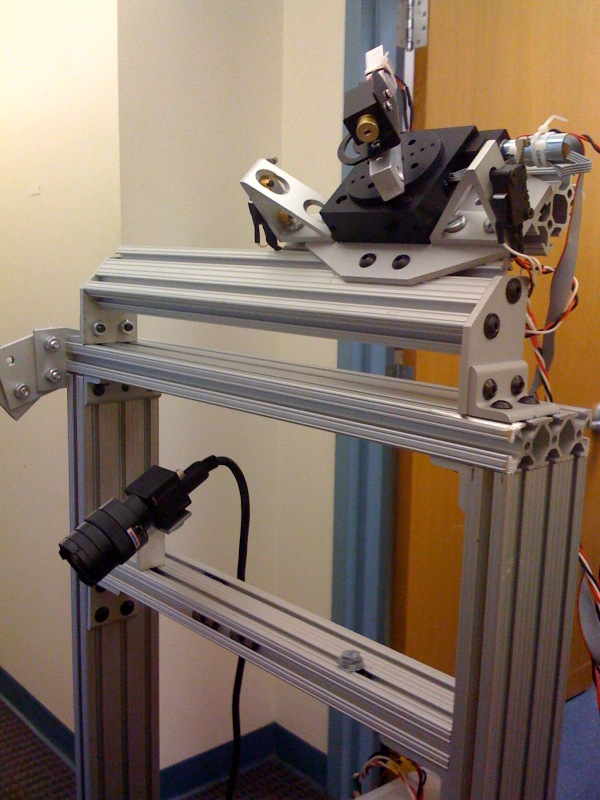
\includegraphics[width=2.5in]{borg2.jpg}
\end{center}
\caption{The scanning hardware on the STAIR 1 robot: the laser and rotary stage are mounted in the upper-right. Images are captured by the camera in the lower-left.}
\label{fig:borg2}
\end{figure}
We used the automatic checkerboard-finding
algorithm and nonlinear solver implemented in OpenCV \cite{bib:opencv} to
estimate the camera intrinsics. To estimate the camera-laser extrinsics, we
start by roughly measuring the translation and rotation by hand. We then scan 
a flat board marked with several points whose relative planar distances have
been carefully measured. The locations of these points in the camera image are
found and recorded. We can then quantify the calibration error: the projected
3D points should be coplanar as well as exhibit the measured distances. We
image this test board from several angles to better cover the workspace of
the scanner. A numerical optimization routine is used to minimize the sum of
the errors while perturbing the parameters, randomly restarting many times to
explore many different local minima.

The resulting calibration holds true except at the extreme edges of the camera
view. We assume this is due to effects of the lens not captured in the standard
radial and tangential distortion models. Away from the edges of the image, 
the scanner shows errors in the 1mm range when imaging flat surfaces such as
doors, desks, and walls.

To calibrate the manipulator to the scanner, we need to define the 6D transform
between the manipulator's base frame and the camera frame. To accomplish this,
we touch the manipulator's end effector to several points on a test board which
are identifiable in the camera frame, logging the manipulator's
forward-kinematics position each time.  We then employ a numerical optimization
routine to improve our hand-measured estimate of the 6D transform.  The
resulting calibration accuracy is approximately 5mm throughout the workspace of
the manipulator.

%%%%%%%%%%%%%%%%%%%%%%%%%%%%%%%%%%%%%%%%%%%%%%%%%%%%%%%%%%%%%%%%%%%%%%%%%%%%%%%%

\section{OBJECT DETECTION}

\begin{figure}[t]
\begin{center}
  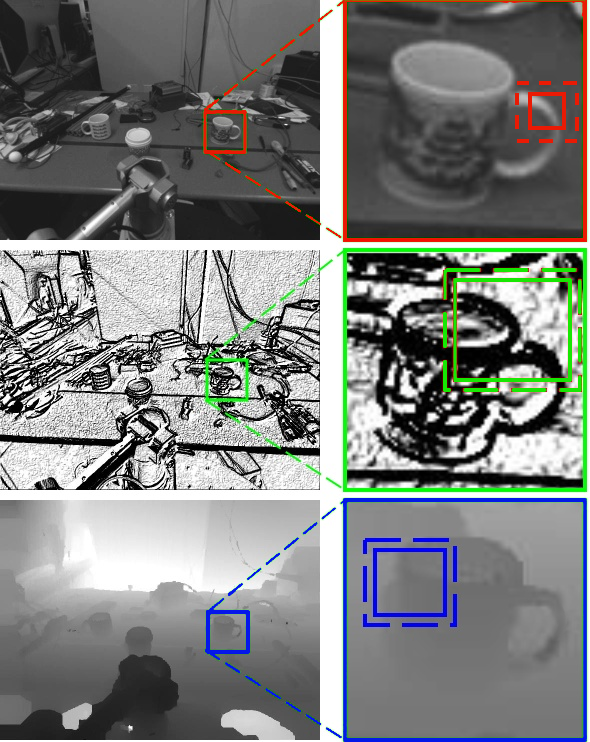
\includegraphics[width=0.95\linewidth]{objdet_mod.png}
  \caption{Image channels considered by the patch-selection algorithm, along with the typical appearance of a coffee mug. A typical patch selected by the system is boxed on right. The larger dashed box indicates the typical 7-pixel window used when finding the maximum patch response. Top (red): intensity image. Middle (green): gradient image. Bottom (blue): depth image.}
  \label{fig:objdet}
\end{center}
\end{figure}


Once the scanner has been calibrated, it can be employed to improve the
performance of object detection. For many robotics applications, this is a
critical subgoal of a larger task: for example, in order to grasp an object it
is first necessary to detect the presence (or absence) of the target object and
localize it in the workspace.

%As discussed in the previous section, the depth information from the scanner is
%defined in the image plane. The absence of an image-to-depthmap registration
%problem (e.g., when the visual light image and depth information are captured
%by separate sensors, requiring the estimation of a 6D transform) is one of the
%key advantages of using triangulation-based methods as opposed to
%time-of-flight methods.

As previously mentioned, the scanner aims to produce a depth estimate for every
pixel. Although the geometry results in the depth being estimated in the image
plane, the information does not lie on a regular grid due to sub-pixel
horizontal interpolation used to estimate the center of the laser stripe.
Furthermore, some regions of the depth image will be more dense than others,
depending on the direction of the surface normal and the distance to the
surface. We thus resample the depthmap using bilinear interpolation to
match the raster of the camera. At this point, the depthmap can be
viewed as another channel in the image.

\subsection{Sliding Windows}

Sliding-window methods attempt to probabilistically match a rectanglar window of
the image with a collection of features local to the window. In our system,
these features are very small ``patches" of the window.

This classifier can be viewed as a black-box which returns a high probability
if the window tightly bounds an instance of the target object class, and a low
  probability otherwise. To perform object detection across an entire image,
  the window is shifted through all possible locations in the image at
  several spatial scales.

We use an extention of the sliding-window approach to combine information from
the visual and depth channels. Similar to the state-of-the-art approach of
Torralba et al. \cite{bib:torralba}, the features used by the probabilistic
classifier are derived from a learned ``patch dictionary." Each patch is a very
small rectangular subregion randomly selected from a set of hand-labeled
training examples. The channels considered are the original (intensity) image,
the gradient image (a transformation of the original image: edges become
bright, flat regions become dark), and the depth map discussed in the previous
section. The patches are drawn separately from these three channels, and 
probabilistically represent the visual appearance (intensity or
edge pattern) or shape (depth profile) of a small region of the object class (Figure \ref{fig:objdet}).

\begin{figure*}[thb]
\begin{center}
  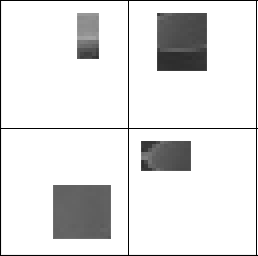
\includegraphics[width=2in]{intensity_patches.png} \quad
  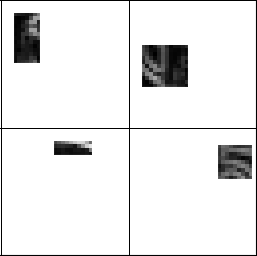
\includegraphics[width=2in]{gradient_patches.png} \quad 
  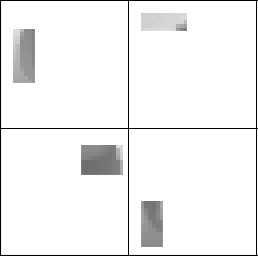
\includegraphics[width=2in]{depth_patches.png}
\end{center}
\caption{Examples of localized patches from the coffee-mug dictionary. Left: Intensity patches. Middle: Gradient patches. Rigth: Depthmap patches.}
\label{fig:mug_classifier}
\end{figure*}

\begin{figure*}[thb]
\begin{center}
  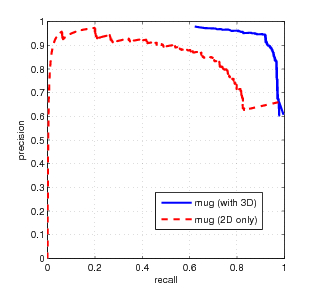
\includegraphics[width=0.32\linewidth]{pr_mug.jpg}
  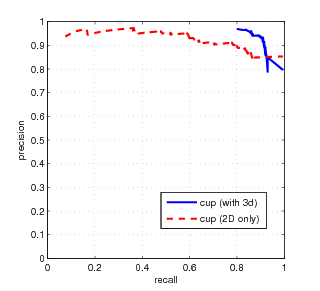
\includegraphics[width=0.32\linewidth]{pr_cup.jpg}
  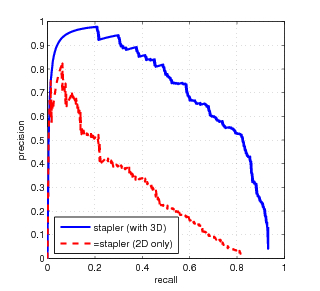
\includegraphics[width=0.32\linewidth]{pr_stapler.jpg}
\end{center}
\caption{Precision-recall curves for mugs (left), disposable cups
  (middle), and staplers (right). Blue solid curve is for our method;
  red dashed curve is for vision only detectors. Scores are computed
  at each threshold by first removing overlapping detections. A
  true-positive is counted if any detection overlaps with our
  hand-labeled groundtruth by more than 50\%. Any detection that does
  not overlap with a groundtruth object of the correct class is
  considered a false-positive. Average Precision measures 11-point
  interpolated area under the recall vs. precision curve. Greater area
  under the curve is better.}
\label{fig:pr_curves}
\end{figure*}

Combined, the patches give a generalized representation of the entire object
class that is robust to occlusion and appearance or shape variation.  When
constructing the dictionary, we record the patch $g$, its location within the
window containing the positive example $w$, and the channel from which it was
drawn $c$ (intensity, gradient, or depth).  A \emph{patch response} for a
particular window is computed by measuring the similarity of the corresponding
region within the window to the stored patch.

More formally, let the image window be represented by three channels
$\{{\cal I}^i, {\cal I}^g, {\cal I}^d\}$ corresponding to intensity,
gradient and depth, respectively. Then the patch response for patch
$p = \left<g, w, c\right>$ is
\[
  \max_{w'} d^c({\cal I}^c, g)
\]
%where $g$ are the patch values, $w$ is the location of the patch
%within the window, $c$ is the channel from which the patch was drawn,
where $d^c()$ is a similarity metric defined for each channel.  To improve
robustness to minor spatial variations, $w'$ is a $7 \times 7$ pixel grid
centered around the original patch location in the training set. This allows
the patches to ``slide" slightly within the window being tested.

We compute similarity between patches using normalized cross-correlation.  For
the intensity and gradient channels we normalize by subtracting the average
(mean) from within the window; for the depth channel we normalize by
subtracting the median depth.

\subsection{Learning the Classifers}

The preceeding discussion assumed that the classifier was already known. In
this section, we discuss how the classifier is built from training data.

For each object class, we learn a binary gentle-boost
classifier~\cite{bib:friedman} over two-split decision stumps in these steps:

\begin{itemize}
\item Construct a training set by cropping positive examples and random negative
windows from our training images.
\item Build an initial patch dictionary by randomly sampling regions from our positive training images, and compute patch responses over our training set.
\item Learn a gentle-boost classifier given these responses.
\item Trim the dictionary to remove all patches that were not selected by boosting.
\item Run the classifier over our training images and augment our set of negative examples with any false-positives found.
\item Repeat the training process with these new negative examples to obtain the final classifier.
\end{itemize}

Since we are learning two-split decision stumps, our classifiers are able to
learn correlations between visual features (intensity patterns and edges) and
object shape (depth). Example patches from a coffee-mug classifier for the
three image channels are shown in Figure \ref{fig:mug_classifier}. This figure
is a typical representation of 12 of the approximately 50 patches selected by
the algorithm.

We performed five-fold cross-validation to evaluate the performance of our
detectors and compare them against state-of-the-art detectors that do not use
depth information. The dataset consisted of 150 images of cluttered office
scenes, with several objects in each scene. We used the same training
procedure (as outlined above) for each detector and report the average
performance over the hold-out sets. Results for coffee mugs, disposable cups,
and staplers are shown in Figure~\ref{fig:pr_curves} and the following
table:%\footnote{Average Precision is calculated as the 11-point interpolated
%area under the recall vs. precision curve.}:
  
\begin{center} \smallskip {\footnotesize \setlength{\tabcolsep}{4pt}
\begin{tabular}{|l|cc|cc|cc|} \hline & \multicolumn{2}{|c|} {\bf{Mug}} &
\multicolumn{2}{|c|} {\bf{Cup}} & \multicolumn{2}{|c|} {\bf{Stapler}} \\ & 3D &
2D & 3D & 2D & 3D & 2D \\ \hline Max. F-1 Score    & 0.932 & 0.798 & 0.922 &
0.919 & 0.662 & 0.371 \\ \hline Average Precision & 0.885 & 0.801 & 0.879 &
0.855 & 0.689 & 0.299 \\ \hline \end{tabular} } \end{center}

In general, the 3D information appears to help eliminate false positives. The
2D detectors seldom miss instances of their trained object class; their typical
problem is instead that they can collect a variety of disparate cues from
shadows or unrelated objects that together match enough of the localized
patches that the sliding-window detector considers it a high-probability
detection. The 3D information can help in this regard: we observe that the
training process often selects relatively large, uniform depth patches.
Effectively, this associates higher probabilities to windows which tightly
bound a single object rather than a collection of several disparate objects.
Since we do not normalize for the depth variation inside a patch, only for its
median, the depth patches also encode a measure of the absolute size of an
object.  These depth cues are not explicitly expressed in the visual-light
image, and as is common in machine learning systems, presenting a richer set of
features to the classifier helps boost performance.

%%%%%%%%%%%%%%%%%%%%%%%%%%%%%%%%%%%%%%%%%%%%%%%%%%%%%%%%%%%%%%%%%%%%%%%%%%%%%%%%
\section{DOOR OPENING}

For many tasks, mobile manipulators operating in home and office environments
need to open and pass through doors. For example, at the end of a workday a
typical office building will have tens or hundreds of closed doors that must be
opened if the robot is to clean the building or search for an item. The ability
to open a door thus needs to be another primitive in the robot's navigation
toolbox, alongside path planning and localization. We summarize our
door-opening system to emphasize the utility of high-resolution 3D sensing for
mobile manipulation.

Door opening requires manipulating the door handle without colliding with the
door. The operation does not allow more than a centimeter or two of positioning
error, as the end effector is continually in close proximity to the (rigid)
door. Thus the door-opening task, like any grasping task where target objects
are identified in a camera, tests not only sensing accuracy but also the
calibration between the sensing system and the manipulator.

Our system uses a hand-annotated map which marks the locations of doors. If the
robot needs to pass through one of the marked doorways, it uses the
triangulation-based laser scanner described in this paper to scan the door.
From this scan, it uses a classifier trained on hundreds of door handles to
localize the handle and classify the door as right-handed or left-handed.  The
robot then drives to within manipulator reach of the door handle, plans a path
to the edge of the handle, and presses on the handle to unlatch it
(Figure \ref{fig:opening_door}). Once the door is unlatched and partially
opened, the robot is able to drive through the door by pushing it fully 
open as its chassis (slowly) comes into contact with the now-unlatched door.

High-resolution point clouds assist in planning collision-free manipulator
paths to the door handle. Some sensing modalities effectively ``low-pass" the
depth map as part of the sensing process. In contrast, the active triangulation
process does not smooth out depth discontinuities, such as those between the
door handle and the door immediately behind it. As a result, the door handle
stands out sharply in the 3D data, making path planning and recognition easier.

%%%%%%%%%%%%%%%%%%%%%%%%%%%%%%%%%%%%%%%%%%%%%%%%%%%%%%%%%%%%%%%%%%%%%%%%%%%%%%%%
\section{INVENTORY-CONTROL EXPERIMENT}

\begin{figure}[t]
\begin{center}
  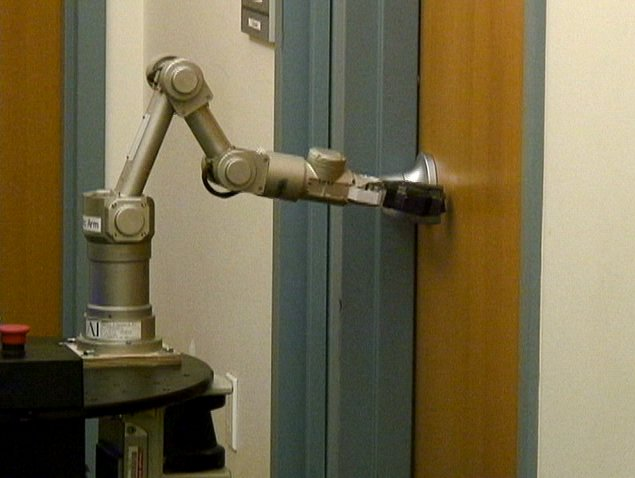
\includegraphics[width=0.95\linewidth]{opening_door.jpg}
\end{center}
\caption{After localizing the door handle in the 3D point cloud, the robot can plan a path to the handle and open the door.}
\label{fig:opening_door}
\end{figure}

\begin{figure}[t]
\begin{center}
  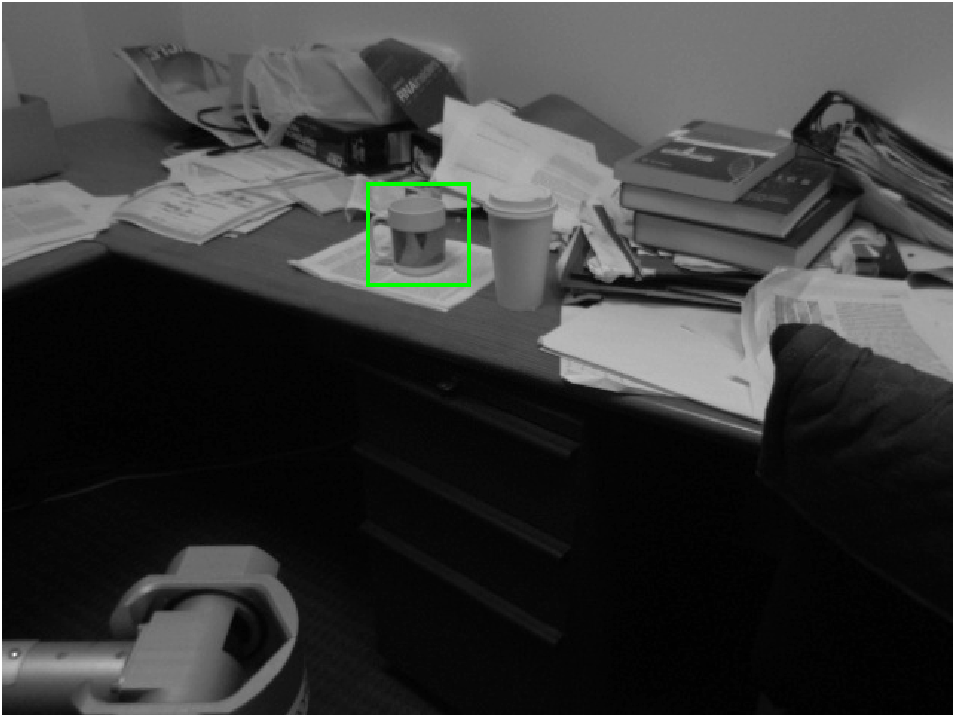
\includegraphics[width=0.8\linewidth]{mug_found3.png}
\end{center}
\caption{Detecting coffee mugs in cluttered environments. The detector correctly ignored the paper cup to the right of the coffee mug.}
\label{fig:mugs_found}
\end{figure}

\begin{figure*}[t]
\begin{center}
  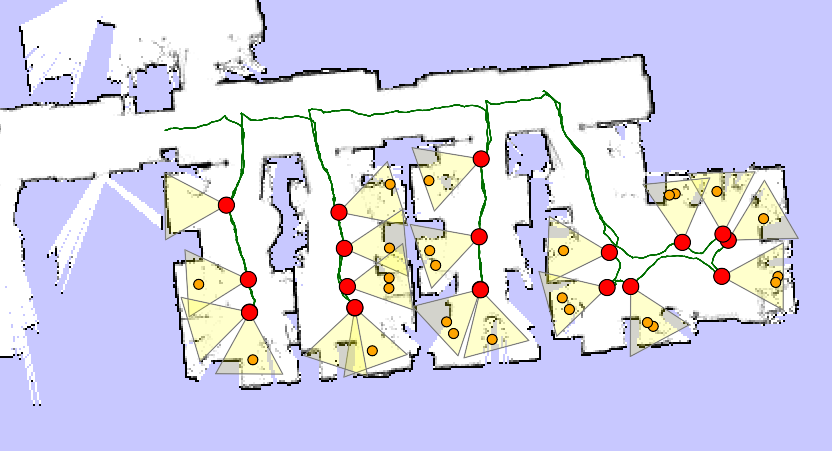
\includegraphics[width=6in]{inventorybot.png}
\end{center}
\caption{The inventory-gathering experiment required autonomous navigation (green track), autonomous door opening, and 20 laser scans of desks in the four offices shown above. The robot position at each scan is shown by the red circles, and the field-of-view of each scan is indicated by the yellow triangles. The
locations of the detected coffee mugs are indicated by the orange circles. This
figure was entirely automatically generated, using the SLAM output for the map
and the localization log for the robot track and sensing positions, which allow
the coffee-mug detections to be transformed into the global map frame.}
%Detecting coffee mugs in cluttered environments: a high rate of false positives (top) occurs even when missing several true positives. In contrast, allowing the algorithm to consider features from the high-resolution depthmap result in no false positives and 100\% detection. None of these examples were used in the training set.}
\label{fig:mugs_found}
\end{figure*}

To evaluate the utility of these two uses of the laser-line triangulation
scanner on our mobile manipulator, we combined the object-detection and 
door-opening algorithms to form an inventory-taking experiment. Such a system
could be envisioned in a future home, perhaps cataloging the locations of
every object in the house at night so that the robot could instantly respond
to human queries about the location of commonly-misplaced objects. Workplace
applications could include inventory-taking in retail stores, safety inspections
in industry, or location verification of movable equipment in, e.g., hospitals.

In our system, a high-level planner sequences a standard 2D navigation stack,
the door-opening system, and the object-detection system, which together allow
the robot to take an inventory of an object class in a cluttered office
building with closed (but unlocked) doors. Our system runs on the ROS software
framework \cite{bib:ros}. A world map was built offline using the GMapping SLAM
toolkit \cite{bib:gmapping} and logged data from the robot's SICK LIDAR and
Segway odometry. The resulting map was hand-annotated to mark the locations of 
doors and desks. The runtime navigation stack is descended from the Player
localization and planning modules, which perform particle-filter localization
and unified object-avoidance and goal-seeking path planning. 

When necessary, control switches to the door-opening system discussed in the
previous section, after which motor control is returned to the 2D navigation
stack.

A sample run of the inventory-gathering system is shown in Figure
\ref{fig:mugs_found}. During this run, there were 25 coffee mugs spread in the
search area. The 3D-enhanced object detector found 24 of them, without any
false positives. Our image-only detector was only able to find 15 of them, and
it found 19 false positives. During the experiment, we also searched the scans
for disposable paper cups. The mug-inventory results and the cup-inventory
results are compared against ground truth in the following tables for both
the integrated 3D detectors and the 2D-only detectors.

\begin{centering}
{\bf{3D-Enhanced Detectors}} \\ \smallskip
\noindent { \footnotesize \begin{tabular}{|l|c|c|c|c|c|}
\hline OBJECT & COUNT & HIT & ERROR & RECALL & PREC. \\
\hline Mug & 25 & 24 & 0 & 0.96 & 1.00 \\
Cup & 10 & 8 & 2 & 0.8 & 0.8 \\
\hline \end{tabular}} \\
\end{centering}

\bigskip
\begin{centering}
{\bf{2D-Only Detectors}} \\ \smallskip
\noindent { \footnotesize \begin{tabular}{|l|c|c|c|c|c|}
\hline OBJECT & COUNT & HIT & ERROR & RECALL & PREC. \\
\hline Mug & 25 & 15 & 19 & 0.6 & 0.441 \\
Cup & 10 & 8 & 4 & 0.8 & 0.67 \\
\hline \end{tabular}} \\
\end{centering}

%%%%%%%%%%%%%%%%%%%%%%%%%%%%%%%%%%%%%%%%%%%%%%%%%%%%%%%%%%%%%%%%%%%%%%%%%%%%%%%%
\newpage
\section{CONCLUSIONS AND FUTURE WORK}

As shown by the PR curves obtained when using the 3D information versus 2D
alone, incorporating high-quality 3D information into the sensing scheme of a
mobile manipulator can increase its robustness when operating in a cluttered
environment. The door-opening task shows that high-quality 3D data can help
accomplish motion planning by accurately sensing the immediate vicinity of the
robot. 

We intend to continue increasing the speed of our 3D triangulation system by
moving to ever-faster camera frame rates. We also intend to explore other 
modalities of obtaining high-accuracy 3D data, and quantify the performance
improvement provided by various depth sensors.

%%%%%%%%%%%%%%%%%%%%%%%%%%%%%%%%%%%%%%%%%%%%%%%%%%%%%%%%%%%%%%%%%%%%%%%%%%%%%%%%

\begin{thebibliography}{99}

\bibitem{bib:eccv}
S. Gould, P. Baumstarck, M. Quigley, A. Y. Ng, and D. Koller, Integrating Visual and Range Data for Robotic Object Detection, {\it European Conference on Computer Vision}, 2008

\bibitem{bib:curbfinder}
C. Mertz, J. Kozar, J. R. Miller, C. Thorpe, Eye-safe Laser Line Striper for Outside Use, {\it IEEE Intelligent Vehicle Symposium}, December 2001

\bibitem{bib:levoy}
M. Levoy, K. Pulli, B. Curless, S. Rusinkiewicz, D. Koller, L. Pereira, M. Ginzton, S. Anderson, J. Davis, J. Ginsberg, J. Shade, D. Fulk, The Digital Michelangelo Project: 3D Scanning of Large Statues, {\it SIGGRAPH}, 2000

\bibitem{bib:nextengine}
http://www.nextengine.com

\bibitem{bib:torralba}
A. Torralba, K. Murphy, W. Freeman, Sharing Visual Features for Multiclass and Multiview Object Detection, {\it NIPS}, 2007

\bibitem{bib:friedman}
J. Friedman, T. Hastie, R. Tibshirani, Additive logistic regression: a statistical view of boosting,
{\it Technical report, Dept. of Statistics, Stanford University}, 1998

\bibitem{bib:li-manufacturing-robot}
J. Li, J. Zhu, Y. Guo, X. Lin, K. Duan, Y. Wang, Q. Tang, Calibration of a Portable laser 3-D Scanner used by a robot and its use in Measurement, {\it Optical Engineering} 47 (1), January 2008

\bibitem{bib:industrial-scanners}
Metris, among other companies, offers precision laser line scanners for manufacturing: \url{http://www.metris.com/products/robot_scanners/k-robot/}

\bibitem{bib:cvpr-88}
J. Jezouin, P. Saint-Marc, G. Medioni, Building an Accurate Range Finder with
off-the-shelf Components, {\it Proceedings of CVPR} 1988, p.195-201

\bibitem{bib:david-scanner}
The ``David Laserscanner" is an example of this technique: \url{http://www.david-laserscanner.com}

\bibitem{bib:door-iros-94}
K. Nagatani, S. Yuta, Designing a Behavior to Open a Door and to Pass Through a Doorway using a Mobile Robot Equipped with a Manipulator, {\it Proceedings of IROS} 1994, p. 847-853.

\bibitem{bib:mars-rover}
L. Matthies, T. Balch, B. Wilcox, Fast Optical Hazard Detection for Planetary Rovers using Multiple Spot Laser Triangulation, {\it ICRA} 1997.

\bibitem{bib:cam-fusion}
J. Zhu, L. Wang, R. Yang, J. Davis, Fusion of Time-of-Flight Depth and Stereo for High Accuracy Depth Maps, {\it Proceedings of CVPR}, 2008.

\bibitem{bib:global-stereo}
J. Sun, N. Zheng, H. Shum, Stereo Matching Using Belief Propagation, {\it IEEE Transactions on Pattern Analysis and Machine Intelligence}, 25 (7), July 2003.

\bibitem{bib:noise-of-3d-cams}
D. Falie, V. Buzuloiu, Noise Characteristics of 3D Time-of-Flight Cameras, {\it International Symposium on Signals, Circuits, and Systems}, 2007.

\bibitem{bib:3d-cam-iros06}
S. May, B. Werner, H. Surmann, K. Pervolz, 3D Time-of-Flight Cameras for Mobile Robotics, {\it IROS}, 2006.

\bibitem{bib:active-vision}
S. Zhang, P. Huang, High-Resolution, Real-Time Three-Dimensional Shape Measurement, {\it Optical Engineering}, 45 (12), December 2006.

\bibitem{bib:ros}
The ROS (Robot Operating System) framework is an open-source, peer-to-peer,
cross-platform message-passing system being jointly developed by Stanford
University and Willow Garage. The ROS distribution wraps many popular code
bases, such as OpenCV, GMapping, the navigation stack from Player, the Stage
and Gazebo simulators, and provides drivers to various pieces of robotics
hardware. ROS is available on Sourceforge. Documentation is available at\\
\url{http://pr.willowgarage.com/wiki/ROS}

\bibitem{bib:gmapping}
G. Grisetti, C. Stachniss, W. Burgard, Improved Techniques for Grid Mapping with Rao-Blackwellized Particle Filters, {\it IEEE Transactions on Robotics}, 2006.

\bibitem{bib:opencv}
\url{http://opencvlibrary.sf.net}


%\bibitem{c1}
%J.G.F. Francis, The QR Transformation I, {\it Comput. J.}, vol. 4, 1961, pp 265-271.

%\bibitem{c2}
%H. Kwakernaak and R. Sivan, {\it Modern Signals and Systems}, Prentice Hall, Englewood Cliffs, NJ; 1991.

%\bibitem{c3}
%D. Boley and R. Maier, "A Parallel QR Algorithm for the Non-Symmetric Eigenvalue Algorithm", {\it in Third SIAM Conference on Applied Linear Algebra}, Madison, WI, 1988, pp. A20.

\end{thebibliography}

\end{document}
